\documentclass[a4paper]{article}
\usepackage[utf8]{inputenc}
\usepackage[german]{babel}
\usepackage{amsmath}
\usepackage{amsfonts}
\usepackage{amssymb}
\usepackage{graphicx}

\author{Merlin Koglin, Timon Vosberg, Merlin Steuer}
\date{Abgabe: 16. Januar 2016}
\title{Lösungen zu Aufgabenblatt 10}


\begin{document}
\maketitle
\tableofcontents

\begin{abstract}
Es wurden die Leistungswerte und Laufzeiten der partdeff-par Implementierung getestet, welche von der Gruppe Koglin, Vosberg, Steuer zu Aufgabenblatt 9 abgegeben wurde. Es wurden außerdem zwei komplette Durchläufe zur Verifikation der Ergebnisse durchgeführt, daher sind in jedem Schaubild zwei Verläufe abgebildet.
\end{abstract}

\newpage

\section{Strong Scaling}
\subsection{Jacobi}
\begin{tabular}{|c|c|c|}
\hline 
Anzahl der Prozesse & Laufzeit in s & Laufzeit in s (2. Durchlauf) \\ 
\hline 
12 & 250.4 & 246.9 \\ 
\hline 
24 & 130.1 & 129.8 \\ 
\hline 
48 & 68.6 & 67.6 \\ 
\hline 
96 & 41.2 & 41.4 \\ 
\hline 
120 & 37.7 & 37.4 \\ 
\hline 
240 & 48.3 & 46.6 \\ 
\hline
\end{tabular} 

Wobei die Anzahl der genutzten Knoten stets $\frac{Anzahl Prozesse}{12}$ entspricht. Auch bei 240 Prozessen wurden jedoch 10 Knoten verwendet. Weiterhin wurden in jedem Lauf 960 Interlines verwendet.

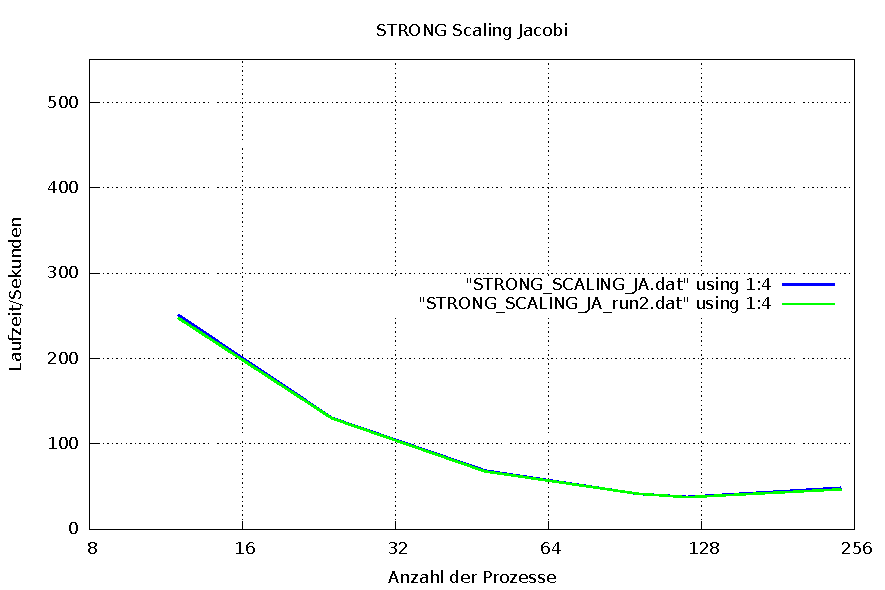
\includegraphics[scale=0.8]{img/STRONG_SCALING_JA_laufzeit.pdf}


\subsection{Gauß-Seidel}
\begin{tabular}{|c|c|c|}
\hline 
Anzahl der Prozesse & Laufzeit in s & Laufzeit in s (2. Durchlauf) \\ 
\hline 
12 & 443.7 & 424.9 \\ 
\hline 
24 & 233.3 & 234.0 \\ 
\hline 
48 & 118.3 & 116.5 \\ 
\hline 
96 & 64.2 & 65.8 \\ 
\hline 
120 & 52.8 & 53.5 \\ 
\hline 
240 & 39.7 & 39.7 \\ 
\hline
\end{tabular} 

Wobei die Anzahl der genutzten Knoten stets $\frac{Anzahl Prozesse}{12}$ entspricht. Auch bei 240 Prozessen wurden jedoch 10 Knoten verwendet. Weiterhin wurden in jedem Lauf 960 Interlines verwendet.

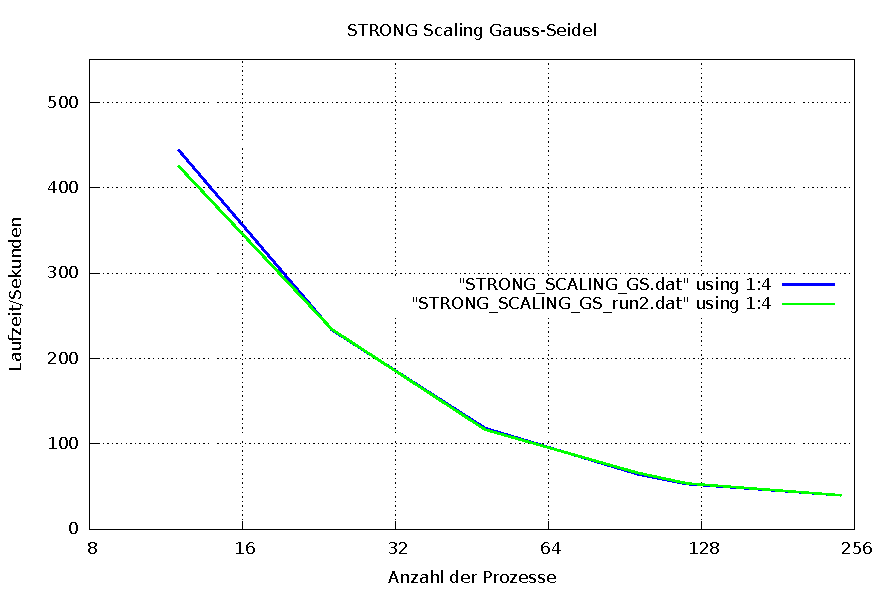
\includegraphics[scale=0.8]{img/STRONG_SCALING_GS_laufzeit.pdf}

\section{Weak Scaling}
\subsection{Jacobi}
\begin{tabular}{|c|c|c|c|c|}
\hline 
Prozesse & Knoten & Interlines & Laufzeit in s & Laufzeit in s (2. Durchlauf) \\ 
\hline 
1 & 1 & 100 & 36.9 & 36.9 \\ 
\hline 
2 & 1 & 141 & 36.9 & 37.2 \\ 
\hline 
4 & 2 & 200 & 38.5 & 38.1 \\ 
\hline 
8 & 4 & 282 & 38.9 & 41.6 \\ 
\hline 
16 & 4 & 400 & 44.4 & 44.6 \\ 
\hline 
24 & 4 & 490 & 42.9 & 44.7 \\ 
\hline 
64 & 8 & 800 & 55.0 & 53.0 \\ 
\hline 
\end{tabular} 

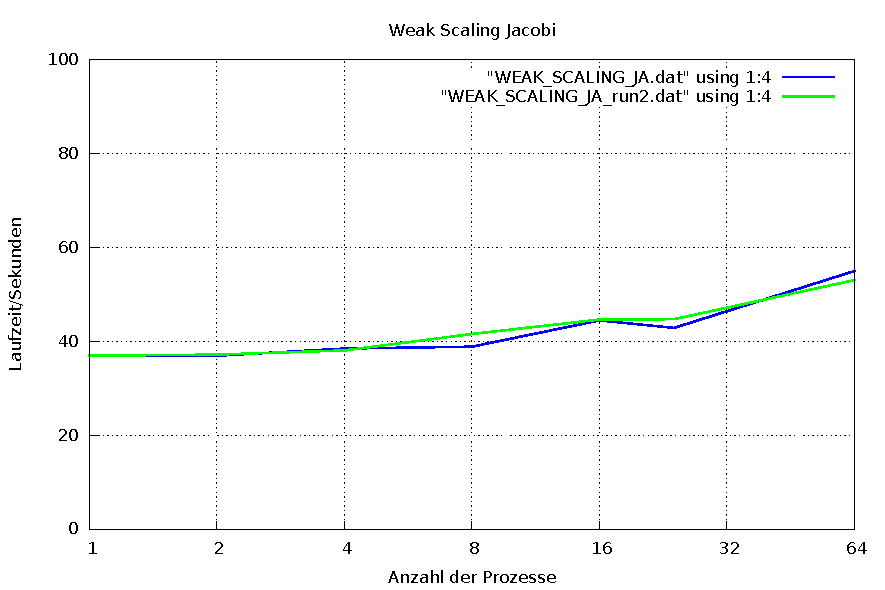
\includegraphics[scale=0.8]{img/WEAK_SCALING_JA_laufzeit.pdf}
\subsection{Gauß-Seidel}
\begin{tabular}{|c|c|c|c|c|}
\hline 
Prozesse & Knoten & Interlines & Laufzeit in s & Laufzeit in s (2. Durchlauf) \\ 
\hline 
1 & 1 & 100 & 37.4 & 37.3 \\ 
\hline 
2 & 1 & 141 & 74.5 & 73.7 \\ 
\hline 
4 & 2 & 200 & 75.3 & 77.6 \\ 
\hline 
8 & 4 & 282 & 76.35 & 78.9 \\ 
\hline 
16 & 4 & 400 & 85.0 & 77.9 \\ 
\hline 
24 & 4 & 490 & 77.6 & 79.5 \\ 
\hline 
64 & 8 & 800 & 92.0 & 91.8 \\ 
\hline 
\end{tabular} 

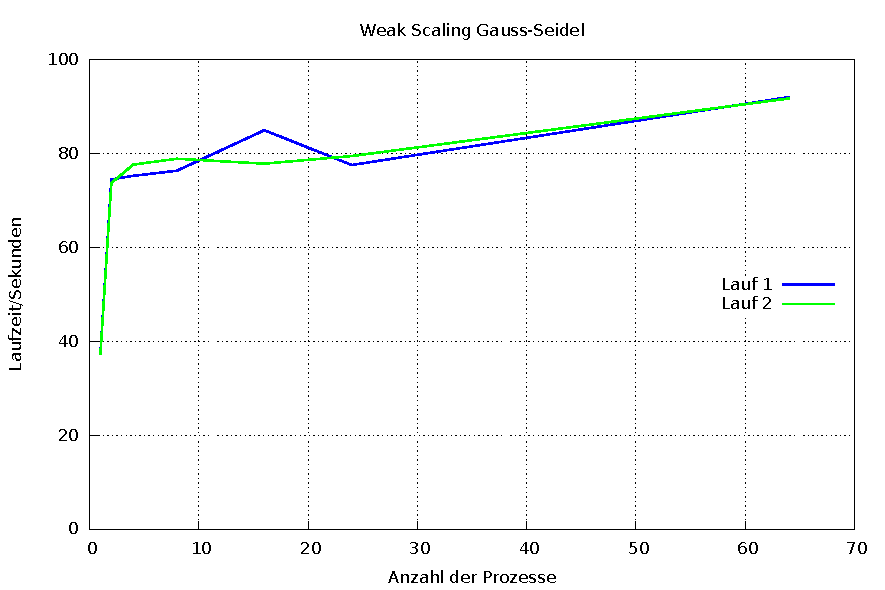
\includegraphics[scale=0.8]{img/WEAK_SCALING_GS_laufzeit.pdf}

\section{Kommunikation und Teilnutzung der Knoten}
\subsection{Jacobi}
\begin{tabular}{|c|c|c|}
\hline 
Knoten (je 10 Proz.) & Laufzeit in s & Laufzeit in s (2. Durchlauf) \\ 
\hline 
1 & 23.7 & 20.0 \\ 
\hline 
2 & 17.1 & 20.9 \\ 
\hline 
3 & 20.2 & 23.7 \\ 
\hline 
4 & 23.0 & 27.1 \\ 
\hline 
6 & 26.8 & 29.5 \\ 
\hline 
8 & 25.9 & 29.7 \\ 
\hline 
10 & 45.1 & 52.3 \\ 
\hline 
\end{tabular} 

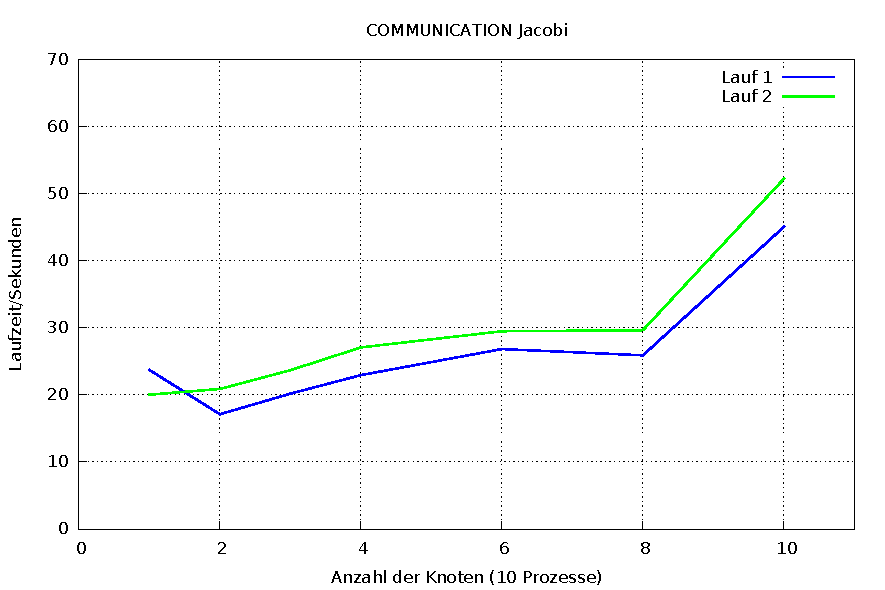
\includegraphics[scale=0.8]{img/COMMUNICATION_JA_laufzeit.pdf}
\subsection{Gauß-Seidel}
\begin{tabular}{|c|c|c|}
\hline 
Knoten (je 10 Proz.) & Laufzeit in s & Laufzeit in s (2. Durchlauf) \\ 
\hline 
1 & 45.0 & 45.1 \\ 
\hline 
2 & 50.6 & 52.4 \\ 
\hline 
3 & 52.6 & 52.5 \\ 
\hline 
4 & 56.7 & 54.4 \\ 
\hline 
6 & 55.9 & 56.3 \\ 
\hline 
8 & 55.3 & 57.1 \\ 
\hline 
10 & 83.4 & 87.8 \\ 
\hline 
\end{tabular} 

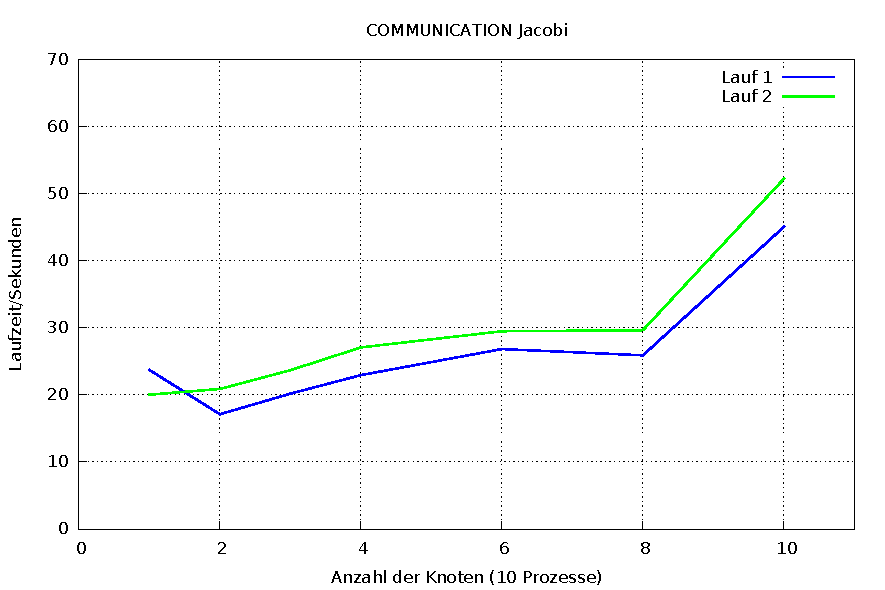
\includegraphics[scale=0.8]{img/COMMUNICATION_JA_laufzeit.pdf}

\end{document}